\section{Architecture}
We take a look at how the system is designed.

\subsection{Actors}
The actors in the system are the ones in table \ref{tab:actors}.
\begin{table}[h!t]
    \caption{Actors in the system.}
    \label{tab:actors}
    \centering
    \begin{tabular}{l p{70mm}}
        \textbf{Name}     & \textbf{Description}                                      \\
        \hline
        User              & The test subject that uses the system.                    \\
        MMPOSE            & The MMPOSE external system used for hand-pose estimation. \\
        Google Speech API & The Google API used for speech-to-text conversion.
    \end{tabular}
\end{table}

% * Requirements.
% \clearpage
\subsection{Requirements}
Requirements are classified based on their priority: \emph{mandatory} or \emph{recommended} and \emph{desirable}.

\begin{table}[h!t]
    \centering
    \caption{\emph{Configure system} requirement.}
    \label{tab:req:configure}
    \centering
    \begin{tabular}{l | p{80mm}}
        \textbf{Id}          & REQ01F                                                                                                      \\
        \textbf{Usecase}     & Configure system                                                                                            \\
        \textbf{Type}        & Functional                                                                                                  \\
        \textbf{Priority}    & Mandatory                                                                                                   \\
        \textbf{Description} & The user should be able to manage which tests will be performed, based on their accessibility requirements.
    \end{tabular}
\end{table}

\begin{table}[h!t]
    \centering
    \caption{\emph{Text recognition} requirement.}
    \label{tab:req:text}
    \centering
    \begin{tabular}{l | p{80mm}}
        \textbf{Id}          & REQ02F                                                                    \\
        \textbf{Usecase}     & Text recognition                                                          \\
        \textbf{Type}        & Functional                                                                \\
        \textbf{Priority}    & Mandatory                                                                 \\
        \textbf{Description} & The user should be able to be subjected to a CAPTCHA-like automated test.
    \end{tabular}
\end{table}

\begin{table}[h!t]
    \centering
    \caption{\emph{Image classification} requirement.}
    \label{tab:req:image}
    \centering
    \begin{tabular}{l | p{80mm}}
        \textbf{Id}          & REQ03F                                                                             \\
        \textbf{Usecase}     & Image classification                                                               \\
        \textbf{Type}        & Functional                                                                         \\
        \textbf{Priority}    & Mandatory                                                                          \\
        \textbf{Description} & The user should be able to be subjected to an image classification automated test.
    \end{tabular}
\end{table}

\begin{table}[h!t]
    \centering
    \caption{\emph{Finger counting} requirement.}
    \label{tab:req:finger}
    \centering
    \begin{tabular}{l | p{80mm}}
        \textbf{Id}          & REQ04F                                                                 \\
        \textbf{Usecase}     & Finger counting                                                        \\
        \textbf{Type}        & Functional                                                             \\
        \textbf{Priority}    & Recommended                                                            \\
        \textbf{Description} & The user should be able to a behavioral finger countng automated test.
    \end{tabular}
\end{table}

\begin{table}[h!t]
    \centering
    \caption{\emph{Word reading} requirement.}
    \label{tab:req:word}
    \centering
    \begin{tabular}{l | p{80mm}}
        \textbf{Id}          & REQ05F                                                                                 \\
        \textbf{Usecase}     & Word reading                                                                           \\
        \textbf{Type}        & Functional                                                                             \\
        \textbf{Priority}    & Recommended                                                                            \\
        \textbf{Description} & The user should be able to be subjected to word reading speech-to-text automated test.
    \end{tabular}
\end{table}

\begin{table}[h!t]
    \centering
    \caption{\emph{Word reading} requirement.}
    \label{tab:req:hearing}
    \centering
    \begin{tabular}{l | p{80mm}}
        \textbf{Id}          & REQ06F                                                                    \\
        \textbf{Usecase}     & Hearing                                                                   \\
        \textbf{Type}        & Functional                                                                \\
        \textbf{Priority}    & Desirable                                                                 \\
        \textbf{Description} & The user should be able to be subjected to a word hearing automated test.
    \end{tabular}
\end{table}

\begin{table}[h!t]
    \centering
    \caption{\emph{Web access} requirement.}
    \label{tab:req:access:web}
    \centering
    \begin{tabular}{l | p{80mm}}
        \textbf{Id}          & REQ07NF                                                              \\
        \textbf{Usecase}     & Web access                                                           \\
        \textbf{Type}        & Non functional                                                       \\
        \textbf{Priority}    & Desirable                                                            \\
        \textbf{Description} & The user should be able to easily access the system through the web.
    \end{tabular}
\end{table}

\begin{table}[h!t]
    \centering
    \caption{\emph{Client access} requirement.}
    \label{tab:req:access:client}
    \centering
    \begin{tabular}{l | p{80mm}}
        \textbf{Id}          & REQ08NF                                                               \\
        \textbf{Usecase}     & Client access                                                         \\
        \textbf{Type}        & Non functional                                                        \\
        \textbf{Priority}    & Desirable                                                             \\
        \textbf{Description} & The user should be able to easily access the system through a client.
    \end{tabular}
\end{table}

\begin{table}[h!t]
    \centering
    \caption{\emph{Portability} requirement.}
    \label{tab:req:portability}
    \centering
    \begin{tabular}{l | p{80mm}}
        \textbf{Id}          & REQ09NF                                                                  \\
        \textbf{Usecase}     & Portability                                                              \\
        \textbf{Type}        & Non functional                                                           \\
        \textbf{Priority}    & Desirable                                                                \\
        \textbf{Description} & The system should work both on desktop and mobile, on the main browsers:
        \begin{itemize}
            \item \emph{Google Chrome} 105.0.5195.102
            \item \emph{Microsoft Edge} 100.0.1185.50
            \item \emph{Mozilla Firefox} 104.0.1
            \item \emph{Opera} 90.0.4480.80
            \item \emph{Safari} 15.6.1
        \end{itemize}
    \end{tabular}
\end{table}

\begin{table}[h!t]
    \centering
    \caption{\emph{Performance} requirement.}
    \label{tab:req:performance}
    \centering
    \begin{tabular}{l | p{80mm}}
        \textbf{Id}          & REQ10NF                                                           \\
        \textbf{Usecase}     & Performance                                                       \\
        \textbf{Type}        & Non functional                                                    \\
        \textbf{Priority}    & Desirable                                                         \\
        \textbf{Description} & The system should be fast enough to be easily usable by the user.
    \end{tabular}
\end{table}

\begin{table}[h!t]
    \centering
    \caption{\emph{Customization} requirement.}
    \label{tab:req:customization}
    \centering
    \begin{tabular}{l | p{80mm}}
        \textbf{Id}          & REQ11NF                                                                                                                                  \\
        \textbf{Usecase}     & Customization                                                                                                                            \\
        \textbf{Type}        & Non functional                                                                                                                           \\
        \textbf{Priority}    & Desirable                                                                                                                                \\
        \textbf{Description} & The system should allow the user to select the appearance of the system, more precisely the following color-palette should be available:
        \begin{itemize}
            \item Light theme.
            \item Dark theme.
            \item Black and white.
            \item Protanopia.
            \item Deuteranopia.
            \item Tritanopia.
        \end{itemize}
    \end{tabular}
\end{table}

\begin{table}[h!t]
    \centering
    \caption{\emph{Security} requirement.}
    \label{tab:req:security}
    \centering
    \begin{tabular}{l | p{80mm}}
        \textbf{Id}          & REQ11NF                                                            \\
        \textbf{Usecase}     & Security                                                           \\
        \textbf{Type}        & Non functional                                                     \\
        \textbf{Priority}    & Mandatory                                                          \\
        \textbf{Description} & The system's tests hould be strong against bot attempting at them.
    \end{tabular}
\end{table}

\begin{table}[h!t]
    \centering
    \caption{\emph{User account} requirement.}
    \label{tab:req:account}
    \centering
    \begin{tabular}{l | p{80mm}}
        \textbf{Id}          & REQ11F                                                                                        \\
        \textbf{Usecase}     & User account                                                                                  \\
        \textbf{Type}        & Functional                                                                                    \\
        \textbf{Priority}    & Recommended                                                                                   \\
        \textbf{Description} & The system should be able to save a user's configuration to avoid having to set it each time.
    \end{tabular}
\end{table}

% * Usecases
\clearpage
\subsection{Use cases}
We show in figure \ref{fig:usecase:diagram} the usecase diagram, tables \ref{tab:uc:system}-\ref{tab:uc:microphone} describes usecases and figures \ref{fig:activity:start}-\ref{fig:activity:microphone} are the respective activity diagrams.

% * Usecase diagram
\subsubsection{Usecase diagram}
\begin{figure}[h!t]
    \centering
    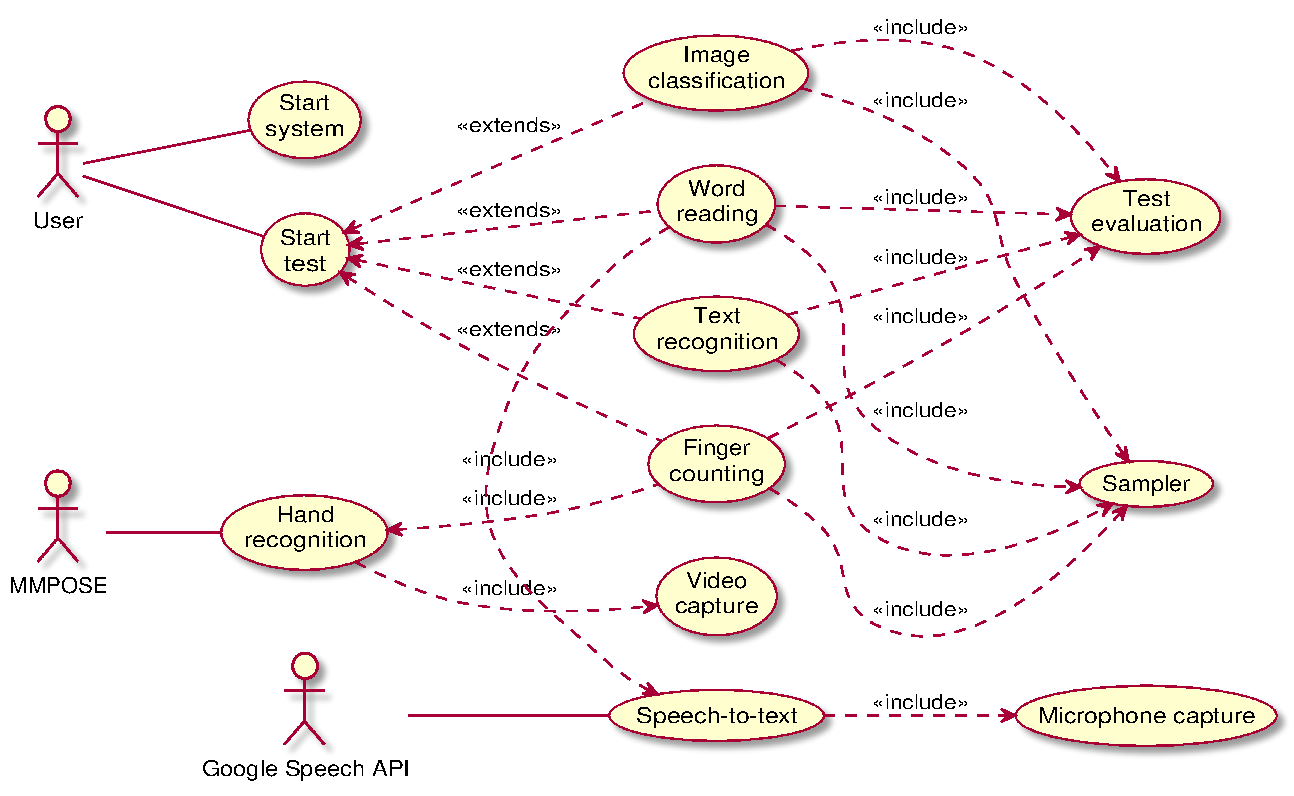
\includegraphics[scale=0.55]{assets/plantuml/pdf/diagram.pdf}
    \caption{Usecase diagrams}
    \label{fig:usecase:diagram}
\end{figure}

% * Usecase tables.
\clearpage
\subsubsection{Usecase descriptions}
\begin{table}[h!t]
    \centering
    \caption{\emph{Start system} usecase.}
    \label{tab:uc:system}
    \centering
    \begin{tabular}{l | p{80mm}}
        \textbf{Id}            & UC01                            \\
        \textbf{Usecase}       & Start system.                   \\
        \textbf{Description}   & The system starts.              \\
        \textbf{Actor}         & User                            \\
        \textbf{Precondition}  & The system has not started yet. \\
        \textbf{Events}        & \begin{enumerate}
            \item The user starts the client.
            \item The user presses the "start" button.
        \end{enumerate}      \\
        \textbf{Postcondition} & The system has started.
    \end{tabular}
\end{table}

\begin{table}[h!t]
    \centering
    \caption{\emph{Start test} usecase.}
    \label{tab:uc:test}
    \centering
    \begin{tabular}{l | p{80mm}}
        \textbf{Id}            & UC02                                                                                \\
        \textbf{Usecase}       & Start test.                                                                         \\
        \textbf{Description}   & The user selects which devices of modes they want to use and gets presented a test. \\
        \textbf{Actor}         & User                                                                                \\
        \textbf{Precondition}  & The system has started.                                                             \\
        \textbf{Events}        & \begin{enumerate}
            \item The user selects which checkboxes they want to be true.
            \item The user presses the "submit" button.
            \item The system shows a test to the user.
        \end{enumerate}                                                          \\
        \textbf{Postcondition} & The user has been submitted to a test.
    \end{tabular}
\end{table}

\begin{table}[h!t]
    \centering
    \caption{\emph{Text recognition} usecase.}
    \label{tab:uc:text}
    \centering
    \begin{tabular}{l | p{80mm}}
        \textbf{Id}            & UC03                                                 \\
        \textbf{Usecase}       & Text recognition.                                    \\
        \textbf{Description}   & The system performs a text recognition test.         \\
        \textbf{Actor}         & -                                                    \\
        \textbf{Precondition}  & The user has expressed to want a test to be started. \\
        \textbf{Events}        & \begin{enumerate}
            \item The system shows a CAPTCHA-like image to a user.
            \item The user selects writes the perceived text into the box.
            \item The user submits the answer.
            \item The system evaluates the output.
            \item The system redirects the user to the home page.
        \end{enumerate}                           \\
        \textbf{Postcondition} & The user has passed or not the test.
    \end{tabular}
\end{table}

\begin{table}[h!t]
    \centering
    \caption{\emph{Image classification} usecase.}
    \label{tab:uc:image}
    \centering
    \begin{tabular}{l | p{80mm}}
        \textbf{Id}            & UC04                                                 \\
        \textbf{Usecase}       & Image classification.                                \\
        \textbf{Description}   & The system performs an image classification test.    \\
        \textbf{Actor}         & -                                                    \\
        \textbf{Precondition}  & The user has expressed to want a test to be started. \\
        \textbf{Events}        & \begin{enumerate}
            \item The system shows an image to a user.
            \item The user selects a class.
            \item The user selects submit.
            \item The system evaluates the output.
            \item The system redirects the user to the home page.
        \end{enumerate}                           \\
        \textbf{Postcondition} & The user has passed or not the test.
    \end{tabular}
\end{table}

\begin{table}[h!t]
    \centering
    \caption{\emph{Finger counting} usecase.}
    \label{tab:uc:finger}
    \centering
    \begin{tabular}{l | p{80mm}}
        \textbf{Id}                 & UC05                                                 \\
        \textbf{Usecase}            & Finger counting.                                     \\
        \textbf{Description}        & The system performs an finger counting test.         \\
        \textbf{Actor}              & -                                                    \\
        \textbf{Precondition}       & The user has expressed to want a test to be started. \\
        \textbf{Events}             & \begin{enumerate}
            \item The system shows a number and to the user.
            \item The system opens the webcam with a coloured region-of-interest.
            \item The user shows the number with their hand inside the RoI.
            \item The system waits for a custom number of correct guesses.
            \item The system redirects the user to the home page.
        \end{enumerate}                           \\
        \textbf{Postcondition}      & The user has passed or not the test.                 \\
        \textbf{Alternative events} & \begin{enumerate}
            \setcounter{enumi}{3}
            \item The user does not show the correct number exceeding the timeout.
        \end{enumerate}
    \end{tabular}
\end{table}

\begin{table}[h!t]
    \centering
    \caption{\emph{Word reading} usecase.}
    \label{tab:uc:word}
    \centering
    \begin{tabular}{l | p{80mm}}
        \textbf{Id}            & UC06                                                 \\
        \textbf{Usecase}       & Word reading.                                        \\
        \textbf{Description}   & The system performs a word reading test.             \\
        \textbf{Actor}         & -                                                    \\
        \textbf{Precondition}  & The user has expressed to want a test to be started. \\
        \textbf{Events}        & \begin{enumerate}
            \item The system shows some words to a user.
            \item The user presses the "Record" button.
            \item The user reads the words aloud.
            \item The system converts the speech to text.
            \item The system matches the converted text with ground truth words.
            \item The system redirects the user to the home page.
        \end{enumerate}                           \\
        \textbf{Postcondition} & The user has passed or not the test.
    \end{tabular}
\end{table}

\begin{table}[h!t]
    \centering
    \caption{\emph{Test evaluation} usecase.}
    \label{tab:uc:evaluation}
    \centering
    \begin{tabular}{l | p{80mm}}
        \textbf{Id}            & UC07                                                                          \\
        \textbf{Usecase}       & Test evaluation.                                                              \\
        \textbf{Description}   & The system evaluates the test performed by the user.                          \\
        \textbf{Actor}         & -                                                                             \\
        \textbf{Precondition}  & The user has performed a test.                                                \\
        \textbf{Events}        & The system compares the user input with the ground truth and returns a value. \\
        \textbf{Postcondition} & -
    \end{tabular}
\end{table}

\begin{table}[h!t]
    \centering
    \caption{\emph{Sampler} usecase.}
    \label{tab:uc:sampler}
    \centering
    \begin{tabular}{l | p{80mm}}
        \textbf{Id}            & UC08                                                                        \\
        \textbf{Usecase}       & Sampler.                                                                    \\
        \textbf{Description}   & The system randomly samples some data that should be presented to the user. \\
        \textbf{Actor}         & -                                                                           \\
        \textbf{Precondition}  & The user has performed a test.                                              \\
        \textbf{Events}        & The system samples data randomly and returns it.                            \\
        \textbf{Postcondition} & -
    \end{tabular}
\end{table}

\begin{table}[h!t]
    \centering
    \caption{\emph{Hand recognition} usecase.}
    \label{tab:uc:hand}
    \centering
    \begin{tabular}{l | p{80mm}}
        \textbf{Id}            & UC09                                               \\
        \textbf{Usecase}       & Hand recognition.                                  \\
        \textbf{Description}   & MMPOSE recognized an hand.                         \\
        \textbf{Actor}         & MMPOSE                                             \\
        \textbf{Precondition}  & The webcam is activated.                           \\
        \textbf{Events}        & MMPOSE recognizes an hand skeleton and returns it. \\
        \textbf{Postcondition} & -
    \end{tabular}
\end{table}

\begin{table}[h!t]
    \centering
    \caption{\emph{Video capture} usecase.}
    \label{tab:uc:video}
    \centering
    \begin{tabular}{l | p{80mm}}
        \textbf{Id}            & UC10                                      \\
        \textbf{Usecase}       & Video capture.                            \\
        \textbf{Description}   & The camera records a video and shows it.  \\
        \textbf{Actor}         & -                                         \\
        \textbf{Precondition}  & The webcam is activated.                  \\
        \textbf{Events}        & The camera shows the live recorded video. \\
        \textbf{Postcondition} & -
    \end{tabular}
\end{table}

\begin{table}[h!t]
    \centering
    \caption{\emph{Speech-to-text} usecase.}
    \label{tab:uc:speech}
    \centering
    \begin{tabular}{l | p{80mm}}
        \textbf{Id}            & UC11                                                          \\
        \textbf{Usecase}       & Speech-to-text.                                               \\
        \textbf{Description}   & The Google Speech API converts a recorded speech to text.     \\
        \textbf{Actor}         & Google Speech API                                             \\
        \textbf{Precondition}  & The microphone is activated.                                  \\
        \textbf{Events}        & The Google Speech API converts speech to text and returns it. \\
        \textbf{Postcondition} & -
    \end{tabular}
\end{table}

\begin{table}[h!t]
    \centering
    \caption{\emph{Microphone capture} usecase.}
    \label{tab:uc:microphone}
    \centering
    \begin{tabular}{l | p{80mm}}
        \textbf{Id}            & UC12                            \\
        \textbf{Usecase}       & Microphone capture.             \\
        \textbf{Description}   & The microphone records a voice. \\
        \textbf{Actor}         & -                               \\
        \textbf{Precondition}  & The microphone is activated.    \\
        \textbf{Events}        & The microphone records a voice. \\
        \textbf{Postcondition} & -
    \end{tabular}
\end{table}

% * Activity diagrams
\clearpage
\subsubsection{Activity diagrams}
\begin{figure}[h!t]
    \centering
    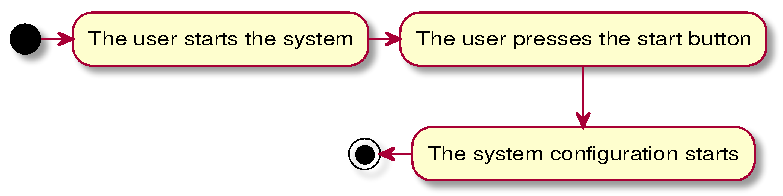
\includegraphics[scale=0.8]{assets/plantuml/pdf/activity/system.pdf}
    \caption{\emph{Start system} activity diagram.}
    \label{fig:activity:start}
\end{figure}

\begin{figure}[h!t]
    \centering
    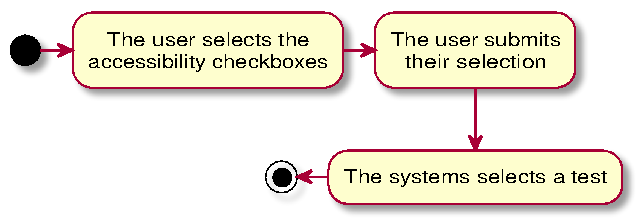
\includegraphics[scale=0.8]{assets/plantuml/pdf/activity/test.pdf}
    \caption{\emph{Start test} activity diagram.}
    \label{fig:activity:test}
\end{figure}

\begin{figure}[h!t]
    \centering
    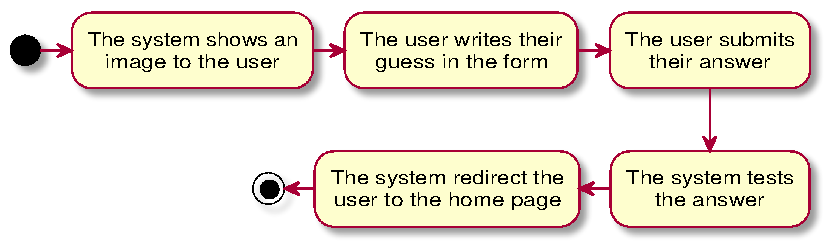
\includegraphics[scale=0.8]{assets/plantuml/pdf/activity/text.pdf}
    \caption{\emph{Text recognition} activity diagram.}
    \label{fig:activity:text}
\end{figure}

\begin{figure}[h!t]
    \centering
    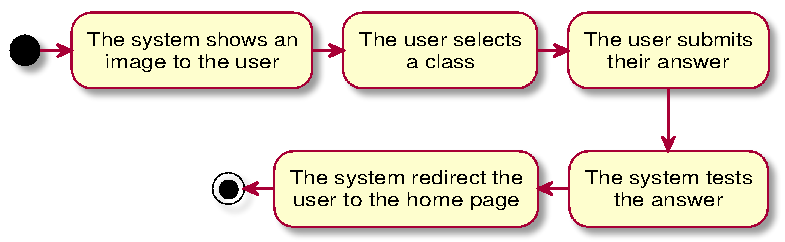
\includegraphics[scale=0.8]{assets/plantuml/pdf/activity/image.pdf}
    \caption{\emph{Image classification} activity diagram.}
    \label{fig:activity:image}
\end{figure}

\begin{figure}[h!t]
    \centering
    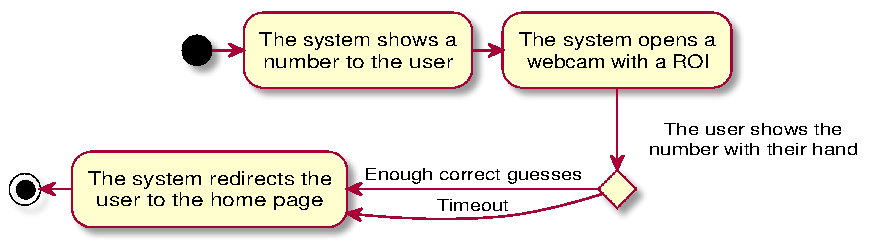
\includegraphics[scale=0.8]{assets/plantuml/pdf/activity/finger.pdf}
    \caption{\emph{Finger counting} activity diagram.}
    \label{fig:activity:finger}
\end{figure}

\begin{figure}[h!t]
    \centering
    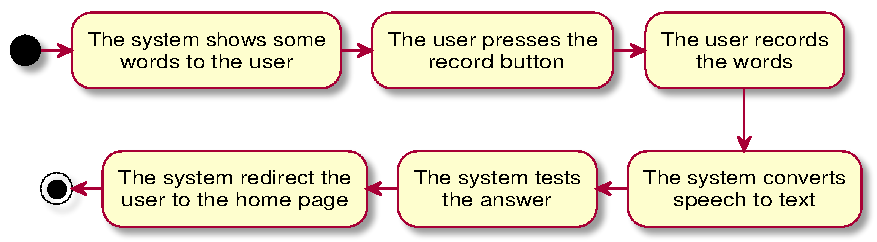
\includegraphics[scale=0.8]{assets/plantuml/pdf/activity/word.pdf}
    \caption{\emph{Word reading} activity diagram.}
    \label{fig:activity:word}
\end{figure}

\begin{figure}[h!t]
    \centering
    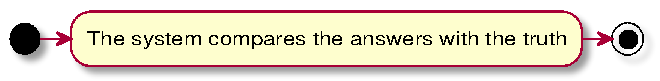
\includegraphics[scale=0.8]{assets/plantuml/pdf/activity/eval.pdf}
    \caption{\emph{Test evaluation} activity diagram.}
    \label{fig:activity:eval}
\end{figure}

\begin{figure}[h!t]
    \centering
    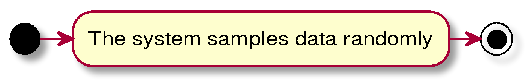
\includegraphics[scale=0.8]{assets/plantuml/pdf/activity/sampler.pdf}
    \caption{\emph{Sampler} activity diagram.}
    \label{fig:activity:sampler}
\end{figure}

\begin{figure}[h!t]
    \centering
    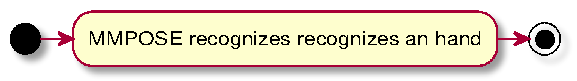
\includegraphics[scale=0.8]{assets/plantuml/pdf/activity/hand.pdf}
    \caption{\emph{Hand recognition} activity diagram.}
    \label{fig:activity:hand}
\end{figure}

\begin{figure}[h!t]
    \centering
    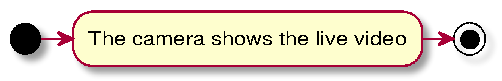
\includegraphics[scale=0.8]{assets/plantuml/pdf/activity/video.pdf}
    \caption{\emph{Video capture} activity diagram.}
    \label{fig:activity:video}
\end{figure}

\begin{figure}[h!t]
    \centering
    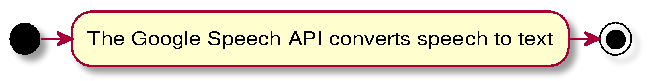
\includegraphics[scale=0.8]{assets/plantuml/pdf/activity/speech.pdf}
    \caption{\emph{Speech-to-text} activity diagram.}
    \label{fig:activity:speech}
\end{figure}

\begin{figure}[h!t]
    \centering
    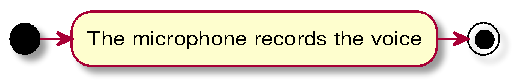
\includegraphics[scale=0.8]{assets/plantuml/pdf/activity/microphone.pdf}
    \caption{\emph{Microphone capture} activity diagram.}
    \label{fig:activity:microphone}
\end{figure}

% * Class diagram
\clearpage
\subsubsection{Class diagram}
\begin{figure}[h!t]
    \centering
    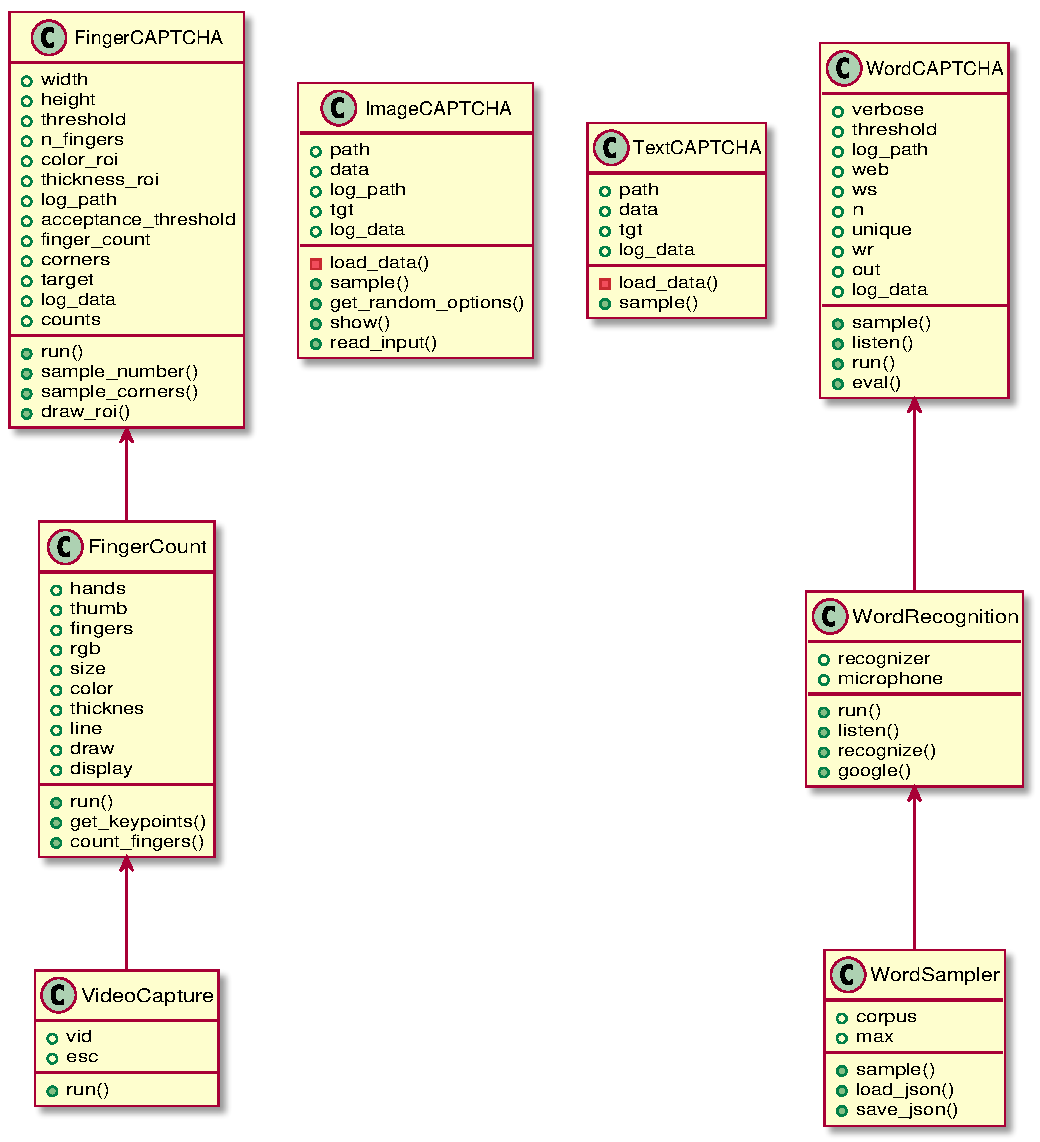
\includegraphics[scale=0.65]{assets/plantuml/pdf/class.pdf}
    \caption{Class diagram.}
    \label{fig:class:diagram}
\end{figure}

% * Sequence diagrams
\clearpage
\subsubsection{Sequence diagrams}
\begin{figure}[h!t]
    \centering
    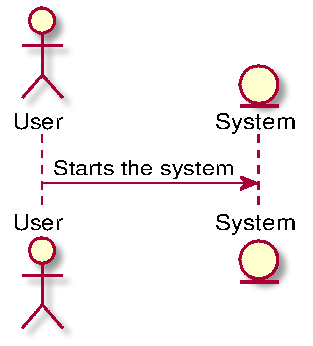
\includegraphics[scale=0.8]{assets/plantuml/pdf/sequence/system.pdf}
    \caption{\emph{Start system} sequence diagram.}
    \label{fig:sequence:start}
\end{figure}

\begin{figure}[h!t]
    \centering
    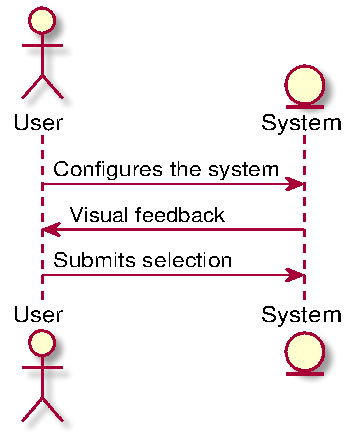
\includegraphics[scale=0.8]{assets/plantuml/pdf/sequence/test.pdf}
    \caption{\emph{Start test} sequence diagram.}
    \label{fig:sequence:test}
\end{figure}

\begin{figure}[h!t]
    \centering
    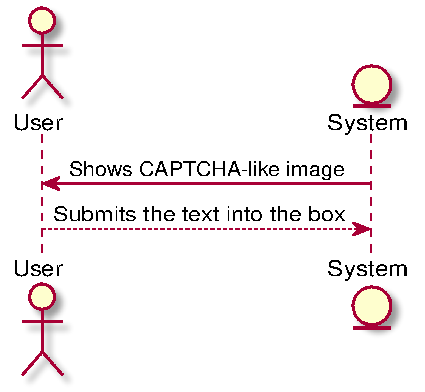
\includegraphics[scale=0.8]{assets/plantuml/pdf/sequence/text.pdf}
    \caption{\emph{Text recognition} sequence diagram.}
    \label{fig:sequence:text}
\end{figure}

\begin{figure}[h!t]
    \centering
    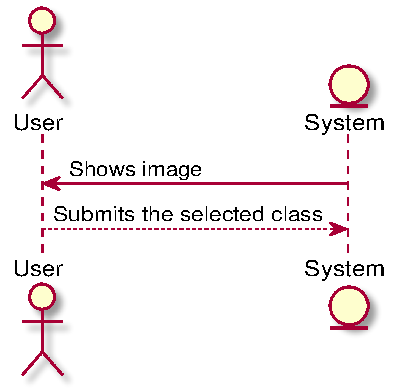
\includegraphics[scale=0.8]{assets/plantuml/pdf/sequence/image.pdf}
    \caption{\emph{Image classification} sequence diagram.}
    \label{fig:sequence:image}
\end{figure}

\begin{figure}[h!t]
    \centering
    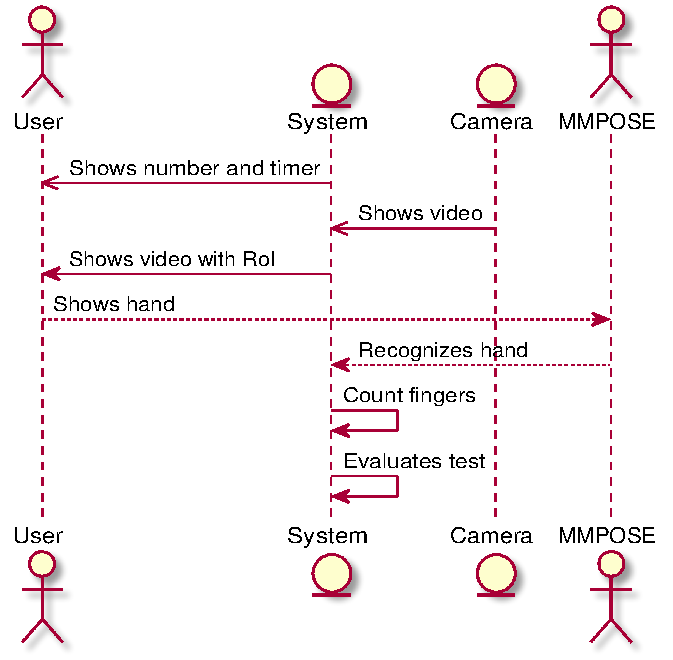
\includegraphics[scale=0.8]{assets/plantuml/pdf/sequence/finger.pdf}
    \caption{\emph{Finger counting} sequence diagram.}
    \label{fig:sequence:finger}
\end{figure}

\begin{figure}[h!t]
    \centering
    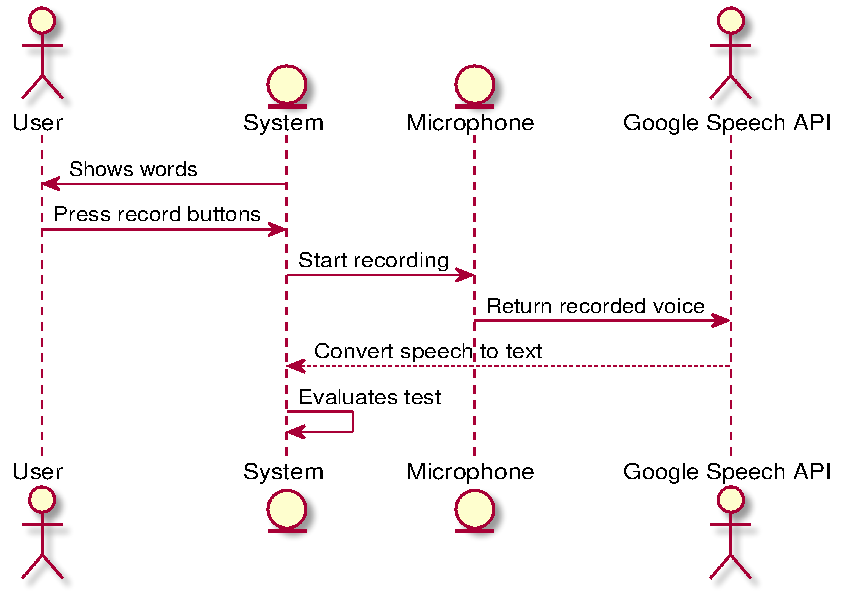
\includegraphics[scale=0.8]{assets/plantuml/pdf/sequence/word.pdf}
    \caption{\emph{Word reading} sequence diagram.}
    \label{fig:sequence:word}
\end{figure}